\documentclass[10pt,aspectratio=169]{beamer}

\usetheme[progressbar=frametitle]{metropolis}

\usepackage{appendixnumberbeamer}
\usepackage{booktabs}
\usepackage[scale=2]{ccicons}

\usepackage{subcaption}
\usepackage{tikz}
\usepackage{minted}
\usepackage{pgfplots}
\usepgfplotslibrary{dateplot}

\usepackage{amssymb}
\usepackage{enumitem}
% Fix beamer with enumitem (https://tex.stackexchange.com/a/24491)
\setitemize{label=\usebeamerfont*{itemize item}%
  \usebeamercolor[fg]{itemize item}
  \usebeamertemplate{itemize item}}
% Add todo list macro in beamer
\newlist{todolist}{enumerate}{2}
\setlist[todolist]{label=$\square$}
\usepackage{pifont}
\newcommand{\cmark}{\ding{51}}%
\newcommand{\xmark}{\ding{55}}%
\newcommand{\done}{\rlap{$\square$}{\raisebox{2pt}{\large\hspace{1pt}\cmark}}%
\hspace{-2.5pt}}
\newcommand{\wontfix}{\rlap{$\square$}{\large\hspace{1pt}\xmark}}



\title{Assessing the Viability of Rust in HPC}
\subtitle{3rd year project presentation}
\author{Edmund Goodman}
\date{\today}
% \institute{University of Warwick}
% \titlegraphic{\hfill\includegraphics[height=1.5cm]{logo.pdf}}


% ================================ %

\begin{document}

\maketitle

\begin{frame}{Agenda}
  \setbeamertemplate{section in toc}[sections numbered]
  \tableofcontents%[hideallsubsections]
\end{frame}

\begin{frame}{Before we begin...}
\begin{itemize}
    \item<1-> The performance analysis section will analyse benchmark runs
    \begin{itemize}
        \item<2-> I'm going to use a tool I built to spawn some benchmark runs
        \item<3-> We will come back and explore them later, once they have completed!
    \end{itemize}
\end{itemize}
\end{frame}

\section{Project Background}

\begin{frame}{The Rust Language \ i}
    \begin{itemize}
        \item Originally developed by Mozilla, and released in 2010
        \item Voted "most loved" programming language
        \item 
    \end{itemize}
% Originally developed by Mozilla, and released in 2010
% Voted "most loved" programming language
% Background in functional languages
% Undefined behaviour prohibition
% Solves lots of bugs
% Recent attention from US govenment (security) / google (1million dollars for C++/rust interop)
\end{frame}

\begin{frame}{The Rust Language \ ii}
    Has been in the news in the last month due to:
    \begin{itemize}
        \item White House Office of the National Cyber Director publishing a press release ``Future Software Should Be Memory Safe'' \cite{PressReleaseFuture2024}  % (February 26th)
        \item Google pledging \$1 million to improve Rust/C++ interoperability\footnote{Including mentioning \texttt{autocxx}, a tool to which I have pull requested integration tests}\cite{ImprovingInteroperabilityRust}  % (February 5th)
    \end{itemize}
\end{frame}

% \begin{frame}{High-Performance Computing}
    % Intro to HPC
    % Intro to Mantevo mini-apps for benchmarking
% \end{frame}

% \begin{frame}{HPCCG}
    % Original mantevo mini-app
    % History
    % What it does
    % Why I selected it
% \end{frame}

% \begin{frame}{P$^3$ HPC - not just performance!}
    % Performance
    %  - This is what we will assess!
    %  - Rust needs to nearly or as fast as C++ to be viable
    % Productivity
    %  - Ergonomic syntax (most loved language...)
    %  - Good, canonical toolchain
    %  - Properties which make writing bug-free code easier
    % Portability
    %  - Rust tooling is very portable!
    %  - not like c++ with 5+ different proprietary compilers with slightly different flags
    %  - still capable of machine-specific optimisations with native architecture flag
% \end{frame}

% \begin{frame}{Existing work}
    % Existence of previous work motivates it as an interesting topic
% % Why it can be misleading
% % Subjectivity
% \end{frame}



\section{Translation Process}

\begin{frame}{C++ vs Rust}
    % The program model is different
    % The domain of valid C++ programs is a strict superset of Rust programs
    % This is helpful, as it means you can't write programs with undefined behaviour
    % This makes translation more difficult
\end{frame}

\begin{frame}{Writing Performant Rust}
    % There are a number of tricks you can do to make Rust more performant
    % Many are enumerated in the Rust Performance Book
\end{frame}

\begin{frame}[fragile]{Fearless Parallelism in Rust}
    \begin{itemize}
        \item<1-> One of Rust's key selling points is ``Fearless Parallelism''
        \begin{itemize}
            \item The borrow checker provides strong guarantees against race conditions/undefined behaviour during parallel execution
        \end{itemize}
        \vspace*{0.5cm}
        \item<2-> The \texttt{rayon} crate provides an even higher-level abstraction for parallelism than \texttt{OpenMP}, with stronger correctness guarantees
        \begin{columns}[T,onlytextwidth]
            \centering
            \column{0.5\textwidth}
            \begin{minted}[escapeinside=||]{rust}
pub fn dot_product(
    lhs: &[f64], rhs: &[f64]
) -> f64 {
    lhs.iter()
        .zip(rhs.iter())
        .map(|(x, y)| x * y)
        .sum()
}
            \end{minted}
            \column{0.5\textwidth}
            \begin{minted}[escapeinside=||]{rust}
pub fn parallel_dot_product(
    lhs: &[f64], rhs: &[f64]
) -> f64 {
    lhs.par_iter()
        .zip(rhs.par_iter())
        .map(|(x, y)| x * y)
        .sum()
}
            \end{minted}
        \end{columns}
    \end{itemize}
\end{frame}

\begin{frame}{Clustered Computing in Rust}
    \begin{itemize}
        \item The Message Passing Interface (MPI) is a common way to distribute work across machines in a HPC computer cluster
        \item MPI has native C++ and FORTRAN implementations of its standard specification
        \item The \texttt{mpi} crate provides bindings from Rust into the C++ implementation
        \begin{itemize}
            \item These bindings are designed to be ``rustic''
            \item They (so far\footnote{I am looking at pull requesting simple examples based on the integration tests}) have quite poor documentation
        \end{itemize}
    \end{itemize}
\end{frame}

\begin{frame}{Translation Workflow}
    % Diagram of loop from translate -> equivalence check -> characterise performance
    % Ease of these three steps constitute criteria for viability of moving from C++ to Rust in HPC
\end{frame}




\section{Equivalence Checking}

\begin{frame}{Equivalence Checking Techniques}
    % End-to-end testing (is fairly effective for chaotic systems like HPCCG)
    %  - Elucidated weird bug in both versions given non-associativity of floating point operations
    % Unit testing
    % Formal methods (refer to Hoare logic with neat example? conclusion as not too helpful)
    % LLVM analysis (just compare some clang decompiled code? conclusion as could be helpful, but high effort to build such a tool)
\end{frame}

\begin{frame}{Novel tool \#1: Polyglotest}
    % Platonic ideal of test-driven development diagram
    % How can we do this within out translation workflow?
    % Pitch idea
    % Show it in action
\end{frame}




\section{Performance Analysis}

\begin{frame}{Testing plan}
    % Implement existing tests (strong/weak scaling scripts)
\end{frame}

% \begin{frame}{Perf/Intel vTune analysis}
% \end{frame}

% \begin{frame}{Overview of results}
% \end{frame}

% \begin{frame}{Novel tool \#2: HPC MultiBench}
% \end{frame}

% \begin{frame}{Returning to the live demo}
% \end{frame}




\section{Project management}
% Can be a little light, but very very required

\begin{frame}{Agile Workflows}
    % Modified picture of a scrum workflow, show how the meeting process with an agenda set maps in

    % Weekly supervisor meetings, which bookend sprints as both a sprint retrospective (discussing work done) and sprint planning (selecting work from the backlog for the next sprint) meeting
    % Weekly meetings have agenda written beforehand, then minutes written up after and submitted to Tabula
    % Benefits of agile methodology
    % - Goal orientation, delivering working software each sprint
    % - Empowerment to adopt initial plan based on new information and ongoing supervisor discussion
\end{frame}

\begin{frame}{Development Tooling}
    % I'm a strong proponent of Git
    % Two major software products tracked in Git/GitHub
    % All deliverables in LaTeX tracked in Git/GitHub
    % Advanced techniques like CI/CD used to enforce code standards
    % Remote backup policy and way to share files between laptop/DCS
\end{frame}

\begin{frame}{Specification Timeline}
    \begin{figure}[h]
        \centering
        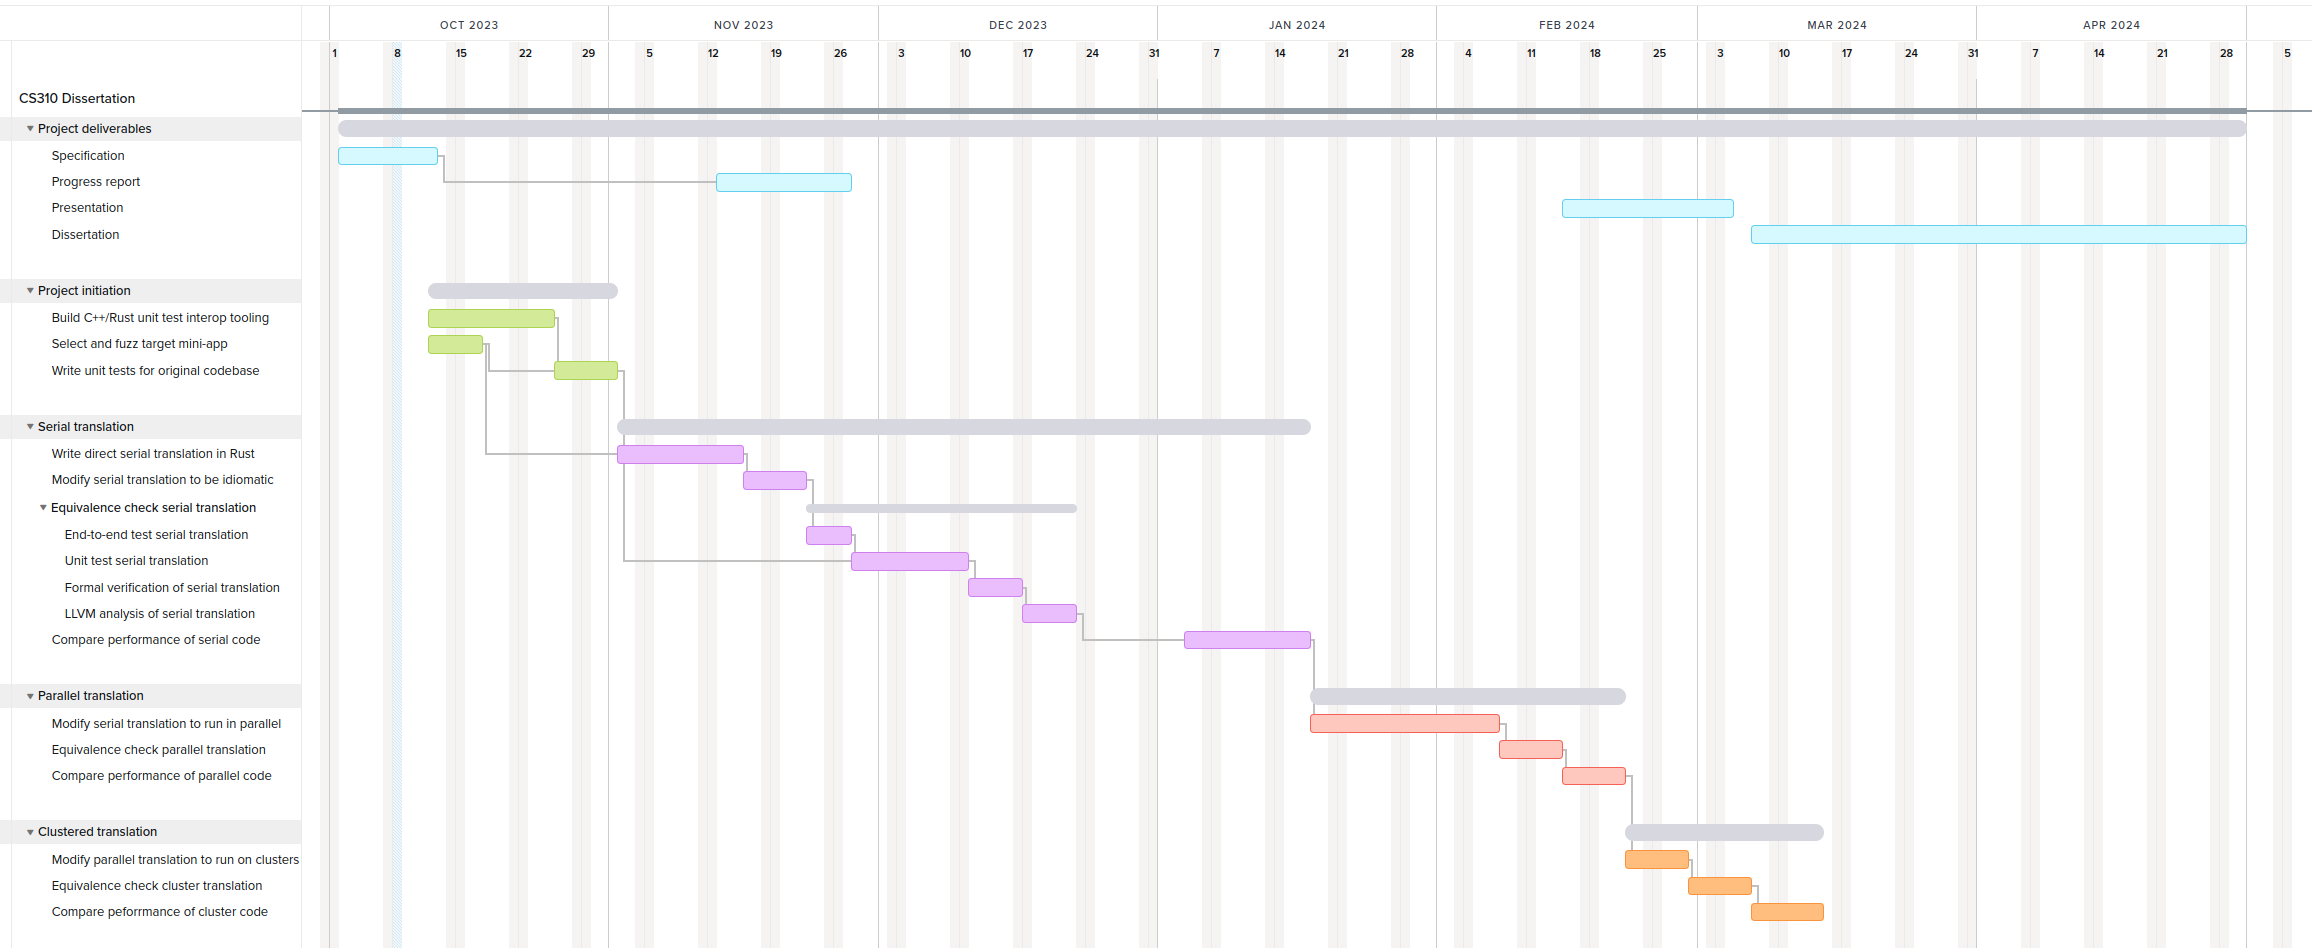
\includegraphics[width=\textwidth]{images/specification_gantt_chart.png}
        \caption{The original timeline from my specification}
        \label{fig:specification_gantt_chart}
    \end{figure}
\end{frame}

\begin{frame}{Actual Timeline}
    \begin{figure}[h]
        \centering
        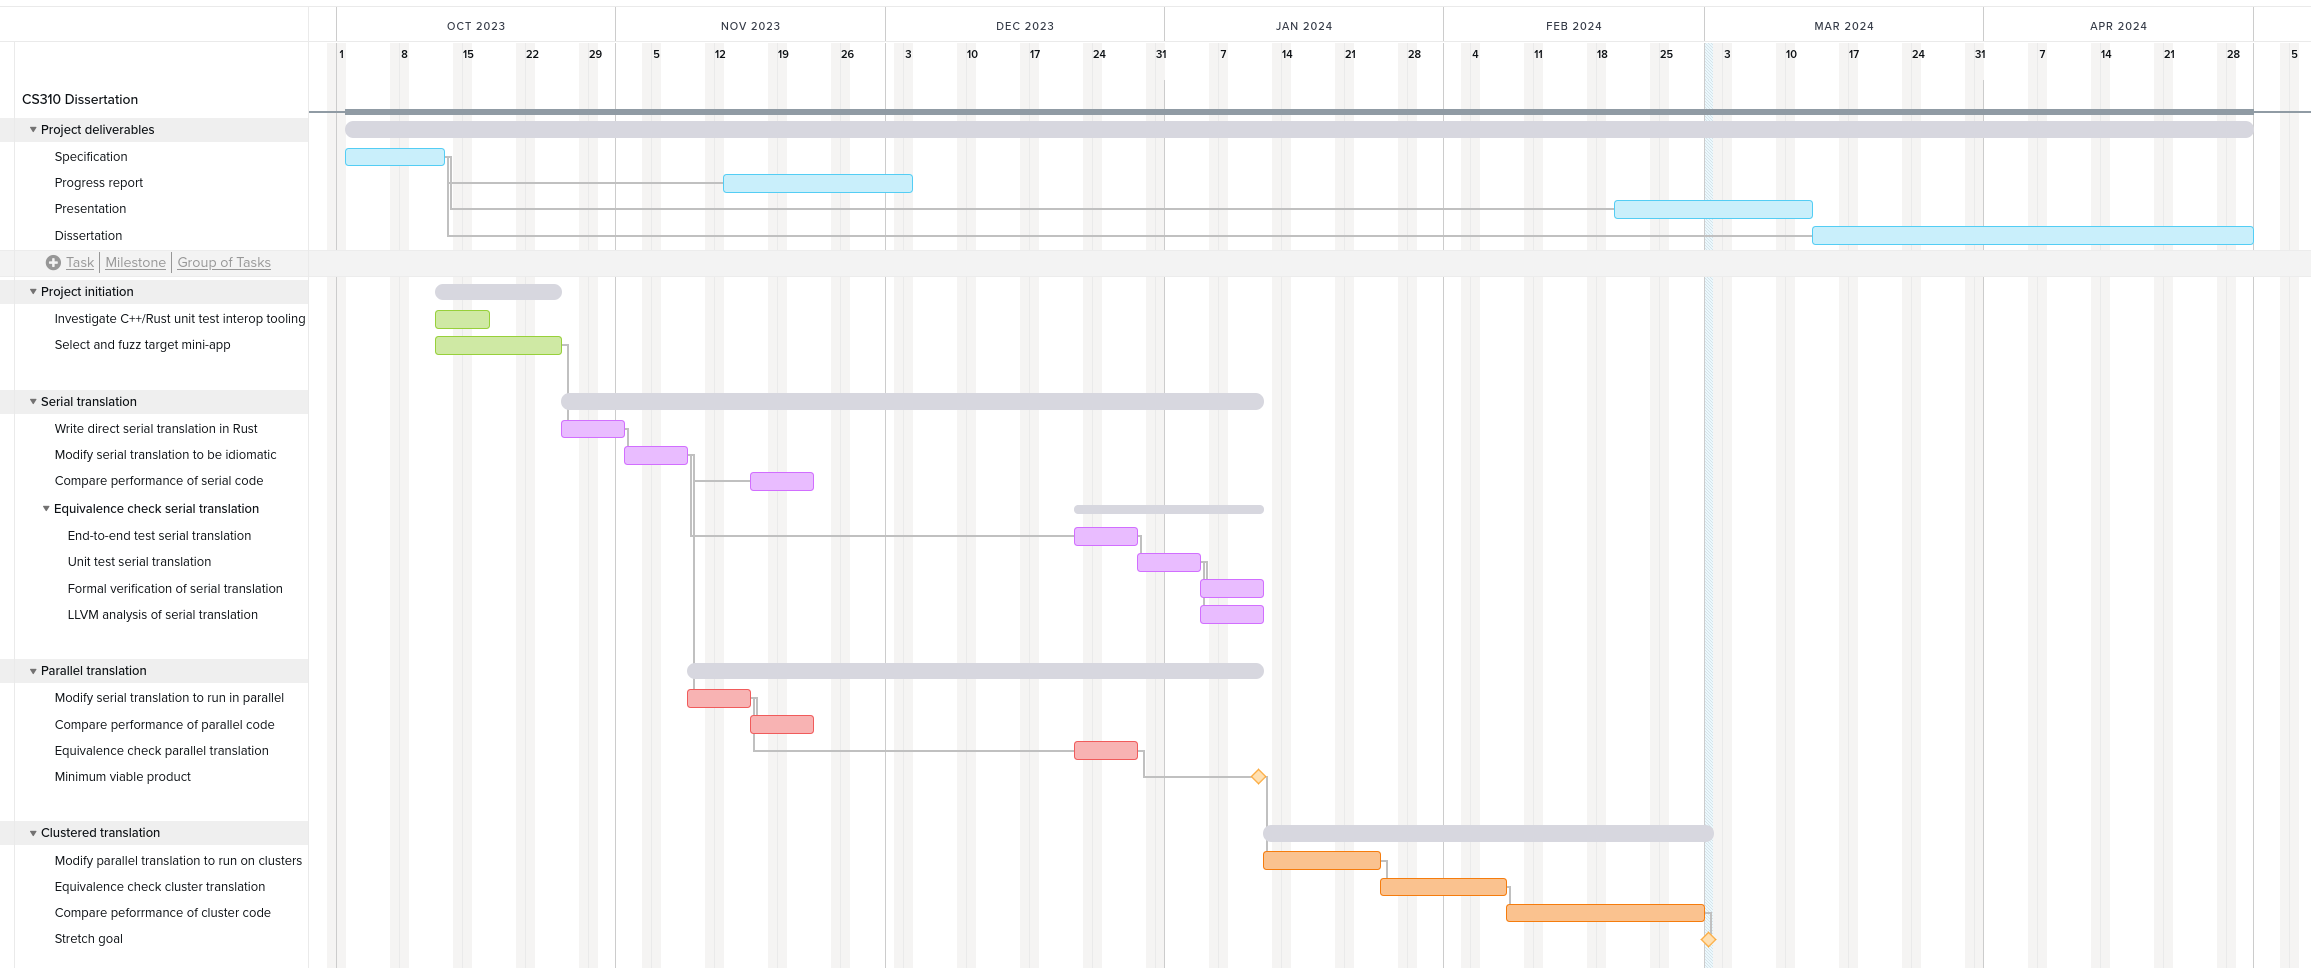
\includegraphics[width=\textwidth]{images/actual_gantt_chart.png}
        \caption{The actual timeline of the project}
        \label{fig:actual_gantt_chart}
    \end{figure}
\end{frame}



\section{Conclusion}

\begin{frame}{Requirements \ i}
    \begin{todolist}
        \item[\done\ \ 1.]
          Select a target mini-app from ECP proxy applications or UK-MAC
          (\textbf{Must have})
        \item[\done\ \ 2.]
          Fuzz test\footnote{an automated testing technique which uses boundary and erroneous test data as inputs, whilst monitoring for resultant undesired behaviour, originally proposed by Miller \textit{et al.} in 1990\cite{millerEmpiricalStudyReliability1990}\cite{liangFuzzingStateArt2018}} the possible mini-apps for memory safety issues using static analysis tooling \cite{stepanovMemorySanitizerFastDetector2015}
          (\textbf{Should have}, \textit{depends on 1})
        \item[\done\ \ 3.]
          Build tooling for running Rust unit tests on C++ code
          (\textbf{Could have})
        \item[\done\ \ 4.]
          Write unit tests for the original C++ version of the
          mini-app
          (\textbf{Should have}, \textit{depends on 1, (3)})
        \item[\done\ \ 5.]
          Write direct translation of serial version mini-app from C++ to Rust
          (\textbf{Must have}, \textit{depends on 1})
        \item[\done\ \ 6.]
          Modify serial version of translated code to be idiomatic Rust \cite{endlerMreIdiomaticrust2023} 
          (\textbf{Should have}, \textit{depends on 5})
    \end{todolist}
\end{frame}

\begin{frame}{Requirements \ ii}
    \begin{todolist}
        \item[\done\ \ 7.]
          Equivalence check serial translated code by comparing results of end-to-end tests with original C++ code
          (\textbf{Must have}, \textit{depends on 5}))
        \item[\done\ \ 8.]
          Equivalence check serial translated code by applying passing C++ unit tests to rust code
          (\textbf{Must have}, \textit{depends on 4, 5})
        \item[\done\ \ 9.]
          Equivalence check serial translated code with limited formal verification techniques
          (\textbf{Could have}, \textit{depends on 5})
        \item[\done\ 10.]
          Equivalence check serial translated code by comparing generated LLVM IR of the C++ and translated Rust versions
          (\textbf{Could have}, \textit{depends on 5})
        \item[\done\ 11.]
          Modify the serial translated code to allow parallel execution
          (\textbf{Must have}, \textit{depends on 5})
        \item[\done\ 12.]
          Equivalence check parallel translated code via all previous techniques
          (\textbf{Must have}, \textit{depends on 7, 8, (9), (10), 11})
        \item[\done\ 13.]
          Carry out a performance analysis of the serial translated Rust code with the original C++ code
          (\textbf{Must have}, \textit{depends on 5})
    \end{todolist}
\end{frame}

\begin{frame}{Requirements \ iii}
    \begin{todolist}
        \item[\done\ 14.]
          Carry out a performance analysis of the parallel translated Rust code with the original C++ code
          (\textbf{Must have}, \textit{depends on 11})
        \item[\done\ 15.]
          Modify the parallel translated code to allow execution across clustered compute resources
          (\textbf{Could have}, \textit{depends on 11})
        \item[\done\ 16.]
          Equivalence check clustered translated code via all previous techniques
          (\textbf{Could have}, \textit{depends on 7, 8, (9), (10), 15})
        \item[\done\ 17.]
          Carry out a performance analysis of the clustered translated Rust code with the original C++ code
          (\textbf{Could have}, \textit{depends on 15})
    \end{todolist}
\end{frame}

\begin{frame}{Evaluation}
    \begin{itemize}
        \item Achieved all specification points, including stretch goal of assessing clustered compute
        \item Successfully ``Assessed the Viability of Rust in HPC'', answering the project question
        \vspace{0.5cm}
        \item \alert{Actively improved} the viability of Rust in HPC, by:
        \begin{itemize}
            \item Developing tools and workflows to assist in translation efforts
            \item Making open source contributions of tests and documentation
        \end{itemize}
    \end{itemize}
\end{frame}


\begin{frame}{Open Source Work}
    \begin{itemize}
        \item Pull requests to existing projects
        \begin{itemize}
            \item Integration tests for array operations to \texttt{autocxx}
            % rs-mpi docs
            % kokkos mini-apps add HPCCG Kokkos version
        \end{itemize}
        \item Repositories to release once project has been assessed
        \begin{itemize}
            \item \texttt{hpccg-rs} A Rust translation of the HPCCG mini-application
            \item \texttt{hpccg-kokkos} A Kokkos translation of the HPCCG mini-application
            \item \texttt{polyglotest} A mini-framework for pure test-driven development of Rust code translated from C++
            \item \texttt{HPC MultiBench} A tool to spawn and analyse Slurm jobs for performance benchmarking
        \end{itemize}
    \end{itemize}
\end{frame}

\begin{frame}{Future work}
\begin{itemize}
    \item<1-> Further research points if the project were longer:
    \begin{itemize}
        \item Translate a second, larger, mini-app such as MiniMD \cite{} or HPCG \cite{}
        \item Extend comparisons to include Rust GPU support
    \end{itemize}
    \vspace{1cm}
    \item<2-> \alert{Publish novel tools developed} as open source repositories
    \begin{itemize}
        \item<3-> If any of them start getting interest, will respond to pull requests/issues as far as possible
    \end{itemize}
    \item<4-> \alert{Aim to submit a paper} based on the project to P3HPC \cite{}
\end{itemize}
\end{frame}




\appendix

\begin{frame}[allowframebreaks]{References}
  % \nocite{*}
  \bibliographystyle{IEEEtran}
  \bibliography{references}
\end{frame}


% \begin{frame}[fragile]{Typography}
%       \begin{verbatim}The theme provides sensible defaults to
% \emph{emphasize} text, \alert{accent} parts
% or show \textbf{bold} results.\end{verbatim}

%   \begin{center}becomes\end{center}

%   The theme provides sensible defaults to \emph{emphasize} text,
%   \alert{accent} parts or show \textbf{bold} results.
% \end{frame}

% \begin{frame}{Font feature test}
%   \begin{itemize}
%     \item Regular
%     \item \textit{Italic}
%     \item \textsc{SmallCaps}
%     \item \textbf{Bold}
%     \item \textbf{\textit{Bold Italic}}
%     \item \textbf{\textsc{Bold SmallCaps}}
%     \item \texttt{Monospace}
%     \item \texttt{\textit{Monospace Italic}}
%     \item \texttt{\textbf{Monospace Bold}}
%     \item \texttt{\textbf{\textit{Monospace Bold Italic}}}
%   \end{itemize}
% \end{frame}

% \begin{frame}{Columns}
%   \begin{columns}[T,onlytextwidth]
%     \column{0.5\textwidth}
%       Items
%       \begin{itemize}
%         \item Milk \item Eggs \item Potatos
%       \end{itemize}

%     \column{0.5\textwidth}
%       Enumerations
%       \begin{enumerate}
%         \item First, \item Second and \item Last.
%       \end{enumerate}
%   \end{columns}
% \end{frame}

% \begin{frame}{Animation}
%   \begin{itemize}[<+- | alert@+>]
%     \item \alert<4>{This is\only<4>{ really} important}
%     \item Now this
%     \item And now this
%   \end{itemize}
% \end{frame}

% \begin{frame}{Figures}
%   \begin{figure}
%     \newcounter{density}
%     \setcounter{density}{20}
%     \begin{tikzpicture}
%       \def\couleur{alerted text.fg}
%       \path[coordinate] (0,0)  coordinate(A)
%                   ++( 90:5cm) coordinate(B)
%                   ++(0:5cm) coordinate(C)
%                   ++(-90:5cm) coordinate(D);
%       \draw[fill=\couleur!\thedensity] (A) -- (B) -- (C) --(D) -- cycle;
%       \foreach \x in {1,...,40}{%
%           \pgfmathsetcounter{density}{\thedensity+20}
%           \setcounter{density}{\thedensity}
%           \path[coordinate] coordinate(X) at (A){};
%           \path[coordinate] (A) -- (B) coordinate[pos=.10](A)
%                               -- (C) coordinate[pos=.10](B)
%                               -- (D) coordinate[pos=.10](C)
%                               -- (X) coordinate[pos=.10](D);
%           \draw[fill=\couleur!\thedensity] (A)--(B)--(C)-- (D) -- cycle;
%       }
%     \end{tikzpicture}
%     \caption{Rotated square from
%     \href{http://www.texample.net/tikz/examples/rotated-polygons/}{texample.net}.}
%   \end{figure}
% \end{frame}

% \begin{frame}{Tables}
%   \begin{table}
%     \caption{Largest cities in the world (source: Wikipedia)}
%     \begin{tabular}{lr}
%       \toprule
%       City & Population\\
%       \midrule
%       Mexico City & 20,116,842\\
%       Shanghai & 19,210,000\\
%       Peking & 15,796,450\\
%       Istanbul & 14,160,467\\
%       \bottomrule
%     \end{tabular}
%   \end{table}
% \end{frame}

% \begin{frame}{Blocks}
%   Three different block environments are pre-defined and may be styled with an optional background color.
  
%   \metroset{block=fill}
%   \begin{block}{Default}
%     Block content.
%   \end{block}
%   \begin{alertblock}{Alert}
%     Block content.
%   \end{alertblock}
%   \begin{exampleblock}{Example}
%     Block content.
%   \end{exampleblock}
% \end{frame}

% \begin{frame}{Math}
%   \begin{equation*}
%     e = \lim_{n\to \infty} \left(1 + \frac{1}{n}\right)^n
%   \end{equation*}
% \end{frame}

% \begin{frame}{Line plots}
%   \begin{figure}
%     \begin{tikzpicture}
%       \begin{axis}[
%         mlineplot,
%         width=0.9\textwidth,
%         height=6cm,
%       ]

%         \addplot {sin(deg(x))};
%         \addplot+[samples=100] {sin(deg(2*x))};

%       \end{axis}
%     \end{tikzpicture}
%   \end{figure}
% \end{frame}

% \begin{frame}{Bar charts}
%   \begin{figure}
%     \begin{tikzpicture}
%       \begin{axis}[
%         mbarplot,
%         xlabel={Foo},
%         ylabel={Bar},
%         width=0.9\textwidth,
%         height=6cm,
%       ]

%       \addplot plot coordinates {(1, 20) (2, 25) (3, 22.4) (4, 12.4)};
%       \addplot plot coordinates {(1, 18) (2, 24) (3, 23.5) (4, 13.2)};
%       \addplot plot coordinates {(1, 10) (2, 19) (3, 25) (4, 15.2)};

%       \legend{lorem, ipsum, dolor}

%       \end{axis}
%     \end{tikzpicture}
%   \end{figure}
% \end{frame}

% \begin{frame}[fragile]{Code Snippets}
%     Code snippets with syntax highlighting can be embedded using then \verb|minted| package:
%     \begin{minted}[escapeinside=||]{haskell}
% newtype Lasagne = Lasagne Int
%     deriving (Show, Num)

% -- The stacking operating can be considered integer 
% -- addition of the number of layers
% instance Semigroup Lasagne where
%     (<>) = (+)
%     \end{minted}
% \end{frame}


\end{document}
